% Poster get from https://github.com/victorsenam/tcc/blob/master/poster/main.tex

\documentclass[final]{beamer}
\usepackage[size=a1,orientation=portrait,scale=1.3]{beamerposter}

\usepackage[brazil]{babel}
\usepackage[utf8]{inputenc}
\usepackage[T1]{fontenc}
\usepackage{framed,graphicx,xcolor} % for shaded box
\usepackage{mathtools}%
\usepackage{tcolorbox} % Para criar bordas elegantes
\usepackage{graphicx}  % Para incluir imagens
\usepackage{caption}   % Para legendas personalizadas
\usepackage{tikz}
\usetikzlibrary{matrix,shapes,positioning,shadows,trees,patterns}

\usepackage[shortlabels]{enumitem}
\usepackage[numbers]{natbib}
\bibliographystyle{plainnat}
  \def\bibfont{\small}

\sloppy

%----------------------------------------------------------------------------------------
%	SHORTCUTS
%----------------------------------------------------------------------------------------
\newcommand{\B}[1]{\mathbb{#1}}
\newcommand{\Cl}[1]{\ensuremath{\mathcal{#1}}}

\newcommand{\sse}{\Leftrightarrow}
\newcommand{\so}{\Rightarrow}
\newcommand{\se}{\Leftarrow}
\newcommand{\rec}{\leftarrow}

\newcommand{\tdots}{\,.\,.\,}

%----------------------------------------------------------------------------------------
%	BEAMER STYL

\usetheme{poster}
\setbeamercolor{block title}{fg=dblue,bg=white}
\setbeamercolor{block body}{fg=black,bg=white}
\setbeamercolor{block alerted title}{fg=dblue,bg=gray!50}
\setbeamercolor{block alerted body}{fg=black,bg=gray!20}
\setbeamercolor{block prob}{fg=black,bg=white}
\setbeamertemplate{caption}[numbered]

%----------------------------------------------------------------------------------------
%	CUSTOM STYLING
%----------------------------------------------------------------------------------------

\newenvironment<>{prob}{
    \begin{beamercolorbox}[sep=1ex,center,dp={1ex}]{block prob}
    \textcolor{dblue}{\textbf{Problema:}}\itshape
}{\end{beamercolorbox}}

\newcommand\halfcol{\column{.46\textwidth}}
\newcommand\onethirdcol{\column{.31\textwidth}}

\newcommand{\Oh}{\mathrm{O}}

% ?????????
\usepackage{subcaption}

\newcommand*\bolinha[1]{\; \tikz[inner sep=.25ex]\node[circle,draw]{#1}; \;}

%----------------------------------------------------------------------------------------
%	POSTER
%----------------------------------------------------------------------------------------

\title{Rainbow Version of Dirac's Theorem: An Algorithmic Approach}
\author{
    Nathan Luiz Bezerra Martins \hspace{200pt} Orientadora: Yoshiko Wakabayashi \\
    \hspace{-885pt}Willian Miura Mori
}
\institute{\vspace{10pt}Departamento de Ciência da Computação,\\
Instituto de Matemática e Estatística, Universidade de São Paulo}

\begin{document}
\begin{frame}[fragile]\centering
  \vspace{-40pt}
  \begin{columns}[T]

    % ----------------------------------------------------------------------------------------
    % PRIMEIRA COLUNA
    % ----------------------------------------------------------------------------------------
    \halfcol
    \vspace{1.5em}
    \begin{alertblock}{Resumo}
      Dada uma coleção $\mathcal{G} = \{G_1, G_2, \ldots, G_n\}$ de grafos de ordem $n \geq 3$, definidos 
      sobre o mesmo conjunto de vértices e que satisfazem a condição de Dirac para cada 
      $G_i$, existe um $\mathcal{G}$-transversal que forma um circuito hamiltoniano, também conhecido
      como Circuito Hamiltoniano Rainbow. Neste trabalho, desenvolvemos um 
      algoritmo eficiente que encontra um Circuito Hamiltoniano Rainbow. Fizemos implementações
      tanto em \texttt{C++} quanto em \texttt{Python} e realizamos testes de desempenho para comparar as duas versões.
      Utilizamos a biblioteca \texttt{manim} para fazer uma animação gráfica do algoritmo.
    \end{alertblock}

    \begin{block}{Conceitos básicos}
        \textbf{Definições principais:}
        \begin{itemize}
          \item Um grafo simples $G$ é um grafo não direcionado sem laços e sem arestas múltiplas, onde $V(G)$ e $E(G)$ são definidos, respectivamente, o conjunto de vértices e o conjunto de arestas desse grafo.
          \item Um \textbf{circuito hamiltoniano} de $G$ é um circuito que visita cada vértice de $G$ exatamente uma vez.
          \item Definimos $\deg(v)$ como o número de vizinhos de um vértice de $v$ em $V(G)$, e $\delta(G) \coloneqq \min\{ \deg(v) : v \in V(G) \}$ como o grau mínimo de um vértice em $G$.
        \end{itemize}
        \vspace{0.5em}
        \textbf{Teorema de Dirac (1952):}
        Se um grafo simples $G$ com $n \geq 3$ vértices tem grau mínimo $\delta(G) \geq \frac{n}{2}$, então $G$ contém um circuito hamiltoniano.
    \end{block}

    \begin{block}{Versões Rainbow de problemas clássicos}
      \textbf{Definição:}

      A versão rainbow de um problema na teoria dos grafos é uma variação 
      que adiciona a restrição de cores à solução desejada. Nesse contexto, o termo rainbow (arco-íris) refere-se a estruturas em um grafo que utilizam 
      elementos provenientes de diferentes subconjuntos, ou arestas com diferentes rótulos ou cores, 
      garantindo que não haja repetições.
      \vspace{1em}

      \textbf{Teorema de Dirac (\textit{Versão Rainbow}):}

      Dada uma coleção $\mathcal{G} = {G_1, G_2, \ldots, G_n}$ de grafos de ordem $n \geq 3$, definidos
      sobre o mesmo conjunto de vértices e que satisfazem a condição de Dirac para cada
      $G_i$, existe um $\mathcal{G}$-transversal que forma um circuito hamiltoniano, também conhecido
      como Circuito Hamiltoniano Rainbow.
      Cada grafo $G_i$ pode ser enxergado como se suas arestas fossem coloridas com a cor $i$.
      
      \begin{center}
            \centering
            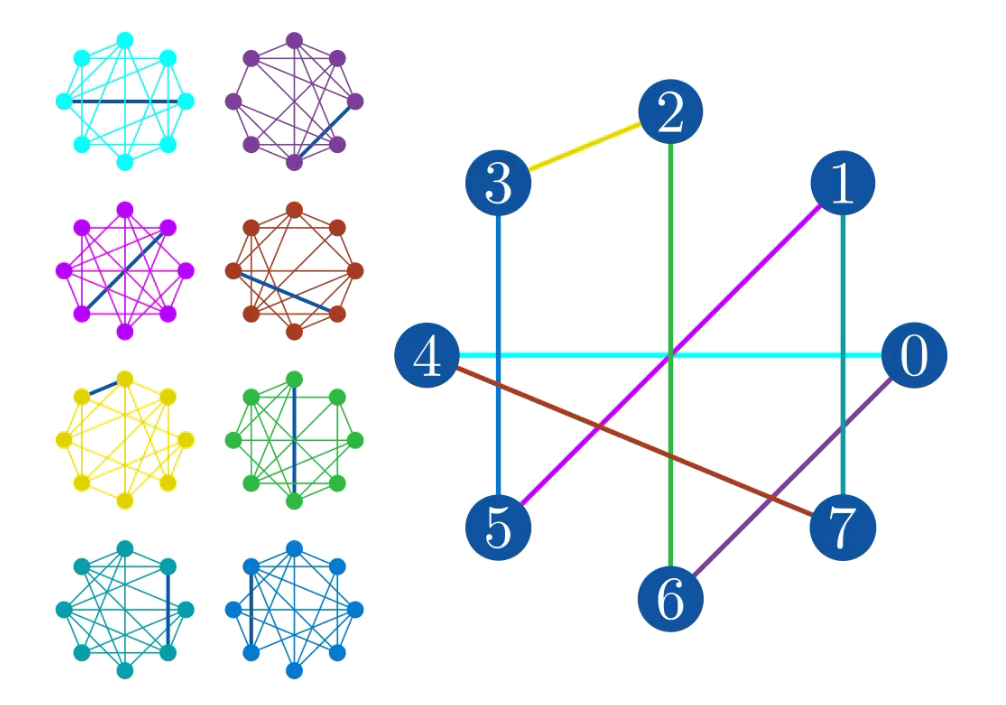
\includegraphics[width=\textwidth]{logos/dirac_rainbow.png}
            \captionof{figure}{Exemplo de um Circuito Hamiltoniano Rainbow para uma coleção de grafos com 8 vértices.}
      \end{center}

      \vspace{1em}
      \textbf{Mais exemplos clássicos:}
      \begin{itemize}
        \item \textbf{Floresta Geradora Mínima Rainbow:} Dado um grafo $G$ e uma coleção de cores, encontre uma floresta geradora mínima que utilize exatamente uma aresta de cada cor.
        \item \textbf{Emparelhamento Perfeito Rainbow:} Dado um grafo bipartido $G$ e uma coleção de cores, encontre um emparelhamento perfeito que utilize exatamente uma aresta de cada cor.
        \item \textbf{Conjunto Independente Rainbow:} Dado um grafo $G$ onde os vértices estão coloridos, encontre o maior conjunto independente de vértices (conjunto de vértices não adjacentes) tal que todas as cores nos vértices do conjunto sejam distintas.
      \end{itemize}

    \end{block}

    % ----------------------------------------------------------------------------------------
    % SEGUNDA COLUNA
    % ----------------------------------------------------------------------------------------
    \halfcol
    \vspace{1.5em}

    \begin{block}{Fluxograma do algoritmo}
      \begin{minipage}[1cm]{0.55\textwidth} % Texto ocupa 55% da largura
        A Figura \ref{fig:flowchart} mostra o fluxograma do algoritmo desenvolvido.
        A ideia principal é, dado um objeto, que pode ser um caminho ou um circuito,
        incrementar esse objeto para um objeto maior.
      \end{minipage}
      \hspace{0.4em}
      \begin{minipage}{0.4\textwidth} % Figura ocupa 40% da largura
          \centering
          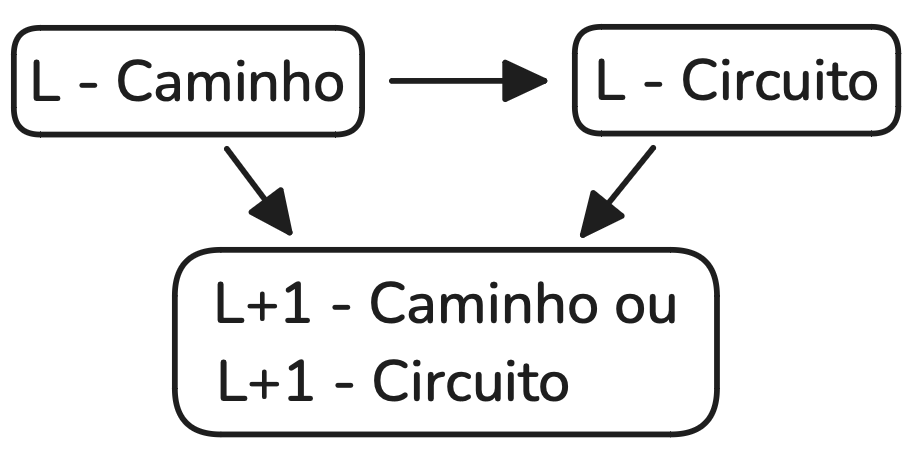
\includegraphics[width=\textwidth]{logos/flowchart.png}
          \captionof{figure}{Fluxograma do algoritmo.}
          \label{fig:flowchart}
      \end{minipage}
    \end{block}

    \begin{block}{Técnicas utilizadas}
      
      Todas as técnicas utilizam fortemente a condição de Dirac para cada grafo.
      \vspace{1em}

      \textbf{Cruzamento:}

      \begin{center}
        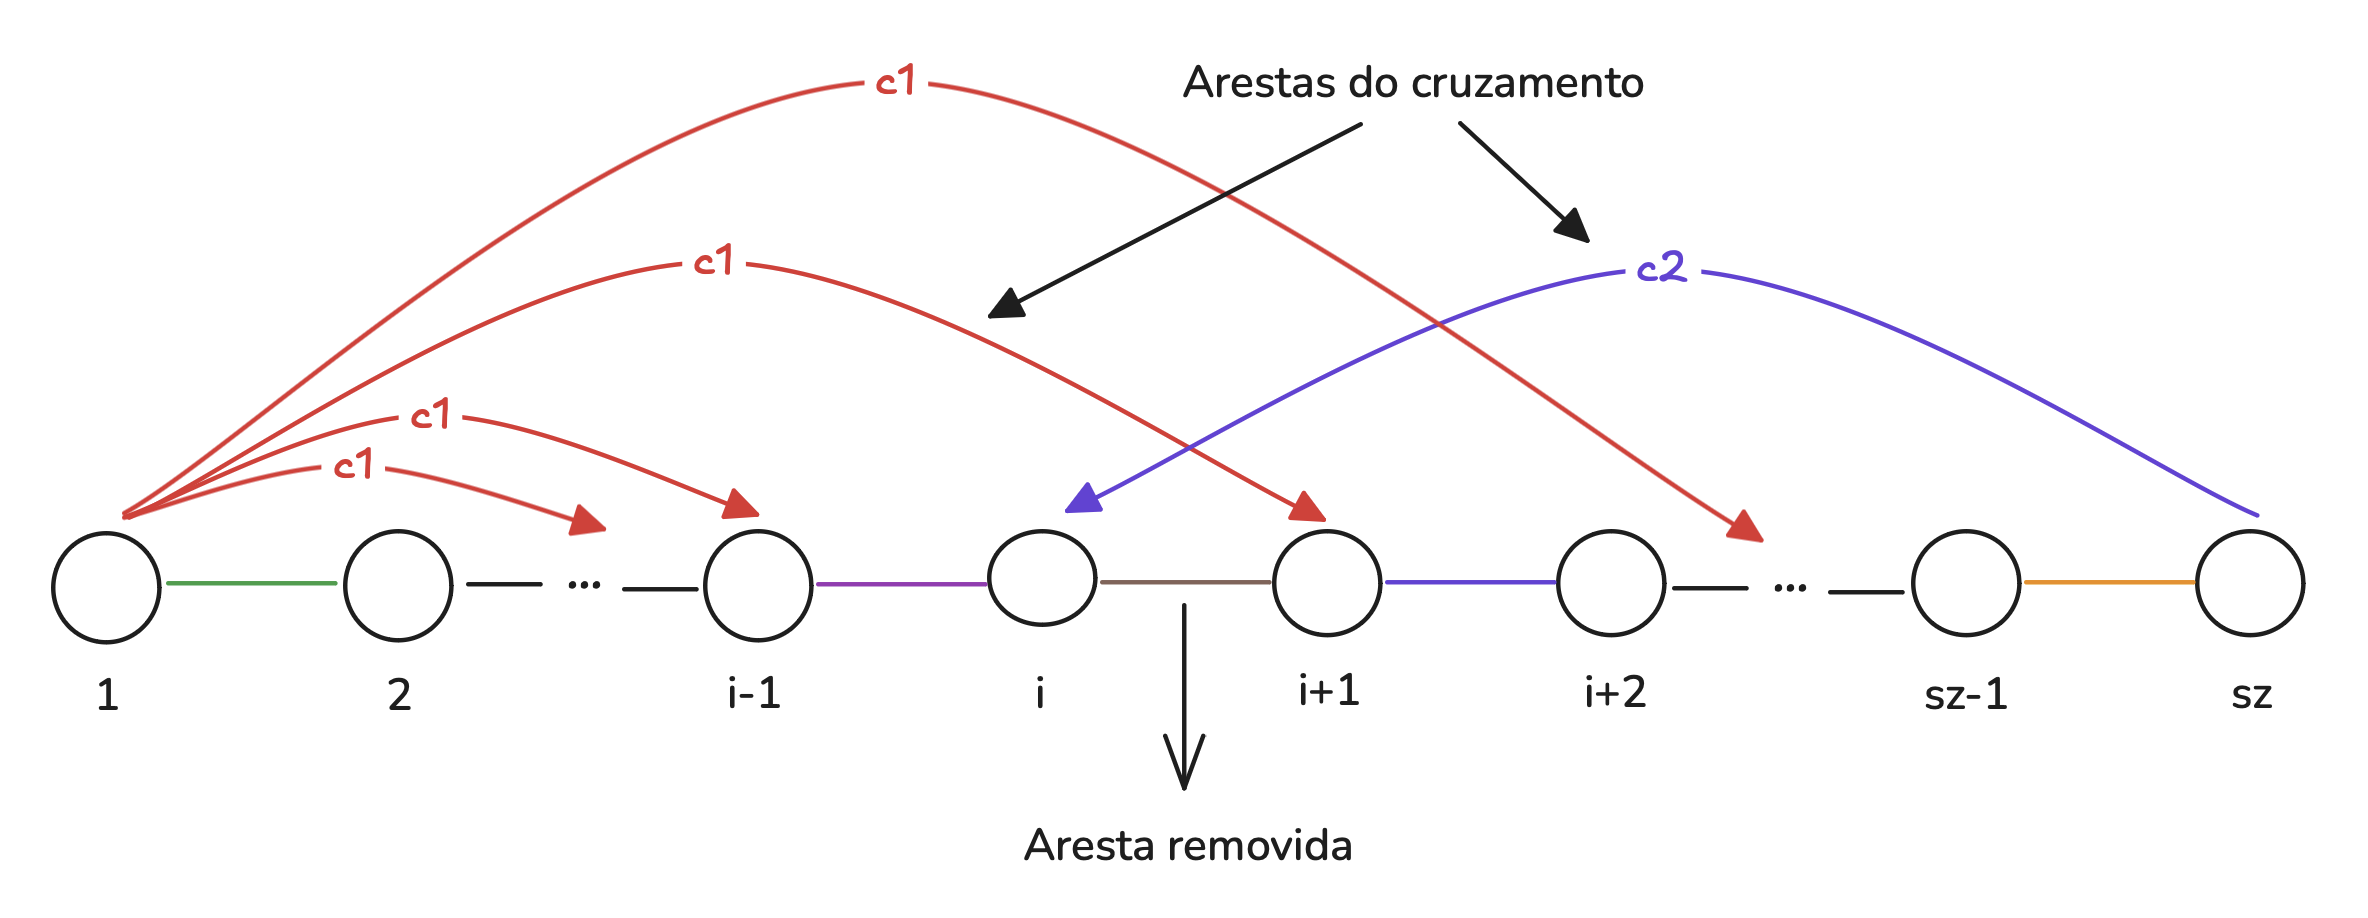
\includegraphics[width=\textwidth]{logos/cruzamento.png}
        \captionof{figure}{Dado um caminho de tamanho $sz$, esta técnica cria um circuito de tamanho $sz+1$.}
      \end{center}

      \textbf{Aresta fora do circuito:}

      \begin{center}
        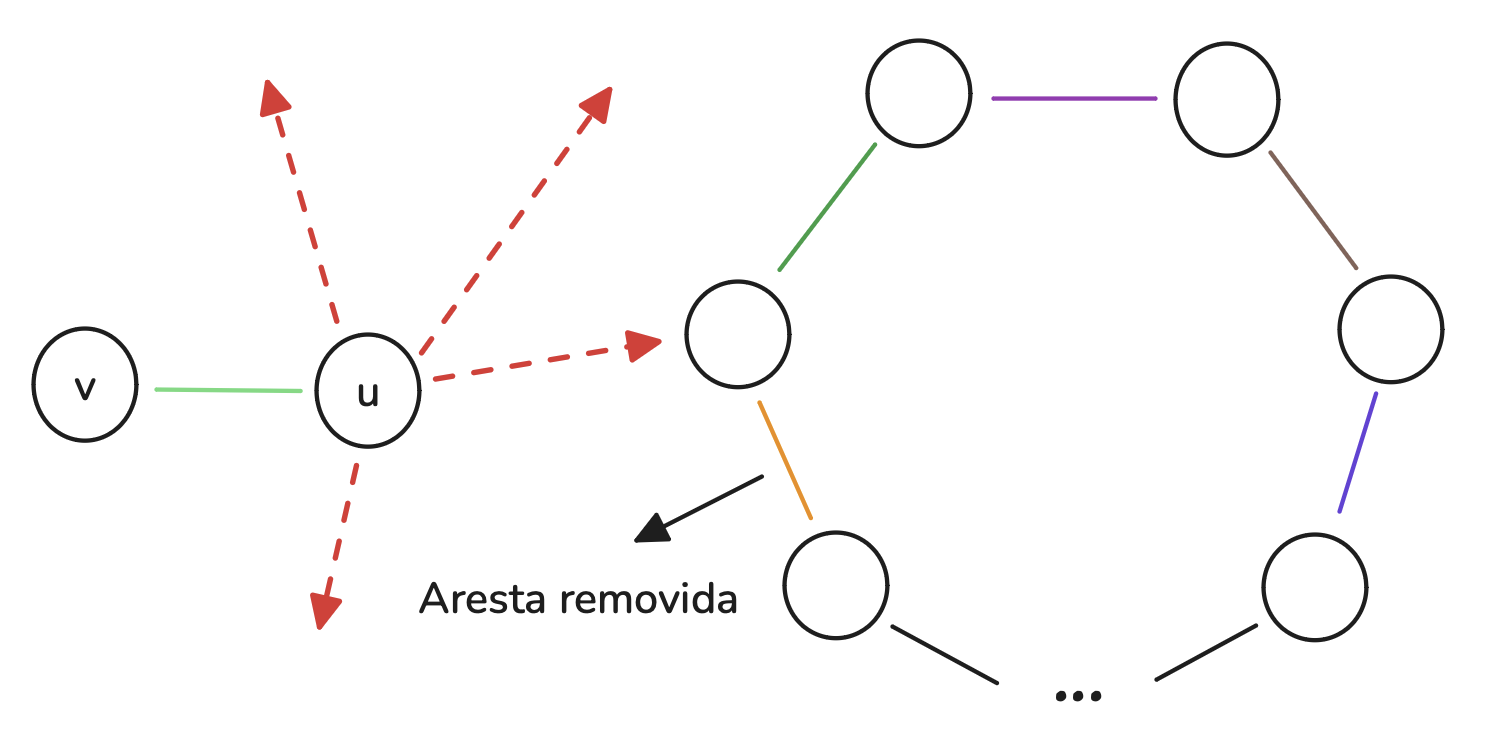
\includegraphics[width=\textwidth]{logos/edge_outside_cycle.png}
        \captionof{figure}{Dado um circuito de tamanho $sz \geq \left \lceil \frac{n}{2} \right \rceil$, esta técnica cria um caminho de tamanho $sz+1$.}
      \end{center}

    \end{block}


    % ----------------------------------------------------------------------------------------
    % TERCEIRA COLUNA
    % ----------------------------------------------------------------------------------------
    % \halfcol

    \begin{block}{Desafios enfrentados}
      \textbf{Criação de uma prova construtiva:}

      A prova original de \textbf{Joos, Kim (2020)} é de natureza não construtiva. Em diversos momentos, 
      o autor solicita que se considere o maior caminho ou circuito \textit{rainbow} e, a partir 
      disso, faz-se uma demonstração. No entanto, ele não explica como encontrar efetivamente 
      esse caminho ou circuito.
      \vspace{0.6em}

      \textbf{Implementação do caso n - 1:}

      Esta é a parte mais difícil do algoritmo. Quase metade do código serve para lidar com esse caso, são muitos detalhes a serem considerados.

      \vspace{0.6em}
      \textbf{Implementação eficiente:}

      A complexidade do algoritmo é da ordem de $\text{O}(n^3)$, em que $n$ é a ordem de $G$. Essa é complexidade é ótima, pois existem $\text{O}(n^3)$ arestas que devem ser consideradas no input.
      
    \end{block}

    \begin{block}{Animação}
      \begin{minipage}{0.55\textwidth} % Texto ocupa 55% da largura
          \raggedright
          Animação demonstrando o algoritmo foram feitas com a biblioteca \texttt{manim} (do canal de Youtube \texttt{3Blue1Brown}) em Python. 
          Um exemplo está disponível no QR Code ao lado.
      \end{minipage}%
      \begin{minipage}{0.4\textwidth} % QR Code ocupa 40% da largura
          \centering
          
\includegraphics[width=0.7\textwidth]{logos/qrcode.png} 
      \end{minipage}
  \end{block}  

  \begin{block}{Referências}
    As referências estão na página da monografia em: \\\textcolor{jblue}{{\url{https://linux.ime.usp.br/~nathanluiz}}}
  \end{block}

  \end{columns}
\end{frame}
\end{document}
